\documentclass[11pt]{article}
\usepackage[a4paper,margin=0.85in]{geometry}
\usepackage[T1]{fontenc}
\usepackage{lmodern,microtype,booktabs,tabularx,amsmath,graphicx}
\usepackage[hidelinks]{hyperref}
\usepackage{caption,tikz}
\usetikzlibrary{arrows.meta,positioning,calc}
\captionsetup{font=small,labelfont=bf}
\setlength{\emergencystretch}{2em}
\setlength{\parskip}{0.3em}
\hypersetup{pdftitle={Improving Automation Discovery with a Workflow Taxonomy - Version 2},pdfauthor={Albert Alises}}
\title{Improving Automation Discovery with a Workflow Taxonomy}
\author{Albert Alises\\n8n\\\texttt{albert.alises@n8n.io}}
\date{9 September 2026\\Version 2}
\begin{document}
\maketitle
\begin{abstract}
We tested whether examples from existing n8n workflows could help an AI agent find work to automate. We first used workflow descriptions to identify tasks that a person could do by hand. We then generated fictional workplace records that showed people doing those tasks: Slack messages, Notion pages, Linear issues, and Salesforce changes.

We used the agent's mistakes on these examples to rewrite its skill: a text file with instructions for finding and checking automation opportunities. We then tested the revised instructions on 57 new fictional companies, each a separate set of activity records with a hidden answer list of tasks the agent could find.

Two language models used the original instructions, the revised instructions, and a short comparison prompt. The revised skill increased average report quality from 44.7\% to 53.0\%, where that score measured the share of proposals in each report that passed checks for evidence, work removal, and correct counts. It also increased the share of known tasks found with valid evidence, called verified task recall, from 28.2\% to 51.7\%. Both gains passed the improvement rule set before the test.

In a second round, we spent ten hours generating and testing more instruction changes. A new test with 116 fictional companies showed higher recall but no clear improvement in report quality, so we kept the skill from the first round. The study supports better task discovery in generated activity, but it does not establish that users will want the proposals or that the automations will save time in practice.

\end{abstract}

\section{The problem: deciding what to automate}
Tools such as n8n help people build automations. Before building one, a person still has to decide which work is worth changing.

That work is often spread across several tools. A request arrives in chat. Someone checks a document, copies fields into a business system, and posts a reply. Because no single record describes the whole task, an agent must connect the records, identify what the person did, and explain how an automation would remove some of that work.

For example, suppose someone receives an invoice by email and copies its details into a payment register. A useful proposal would describe how to extract those details, check for an existing entry, and create the new row. A reminder to enter the invoice would leave the copying with the person.

The agent must also count the work correctly. Three messages about one invoice are evidence of one invoice being processed, not of three separate invoices, so a proposal that counts messages can overstate the opportunity.

In a live product, the agent also needs to know the user's role, goals, and access to data, and the user must decide whether the proposed change is useful. This study tested a narrower question: \textbf{given a fixed set of workplace records, can better instructions help an agent find tasks and support its proposals with the right evidence?}

We developed the skill through two rounds of one study: the first produced a version that passed a separate test, and the second attempted to improve it. Each round used new cases for its final test.

\begin{figure}[htbp]
\centering
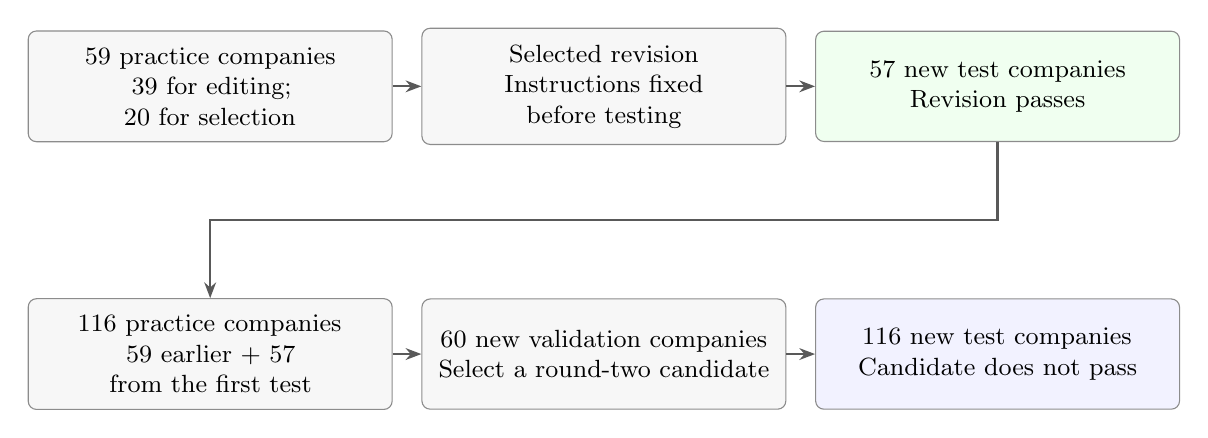
\begin{tikzpicture}[
  box/.style={draw=black!45,rounded corners=3pt,fill=black!3,
    text width=4.2cm,minimum height=1.4cm,align=center,inner sep=6pt,font=\small},
  flow/.style={-{Stealth[length=2mm]},thick,draw=black!65}]
\node[box] (practice) at (0,0) {59 practice companies\\39 for editing; 20 for selection};
\node[box] (revision) at (5,0) {Selected revision\\Instructions fixed before testing};
\node[box,fill=green!6] (first) at (10,0) {57 new test companies\\Revision passes};
\node[box] (secondpractice) at (0,-3.4) {116 practice companies\\59 earlier + 57 from the first test};
\node[box] (selection) at (5,-3.4) {60 new validation companies\\Select a round-two candidate};
\node[box,fill=blue!5] (second) at (10,-3.4) {116 new test companies\\Candidate does not pass};
\draw[flow] (practice) -- (revision);
\draw[flow] (revision) -- (first);
\draw[flow] (secondpractice) -- (selection);
\draw[flow] (selection) -- (second);
\draw[flow] (first.south) -- (10,-1.7) -- (0,-1.7) -- (secondpractice.north);
\end{tikzpicture}
\caption{Two rounds of one study. The second round reused the first test for practice, then used new companies for selection and testing. The first-round skill was retained.}
\end{figure}

\section{Step one: create realistic task examples}
\subsection{Start with work that n8n workflows already perform}
We used a private collection of n8n workflow descriptions, each saying what an automation did, together with business categories and information about successful executions.

The categories formed a \textbf{taxonomy}: a way to group workflows by the kind of work they served. Labels for business functions, such as sales or finance, help explain this idea, because they let us select a mix of work instead of drawing every example from one business area.

We selected groups of workflows with sustained successful use across several business areas. Execution records gave us evidence that these automations had been used, though they did not prove that a person had done the same work before automation, or that another user would want it automated.

One selected group of workflows supplied the starting material for one fictional company. The company name and its workplace activity were generated for the study, so a test company was a collection of related examples, not a real company being observed.

\subsection{Turn a workflow description into a possible human task}
A language model read each selected workflow description and wrote a possible task that a person could perform. A model from the other model family checked that task against the same description, testing whether the description supported the operation and whether the task duplicated another one.

The following example explains the conversion. It is an illustration, not a quoted customer record.

\begin{center}
\small
\setlength{\tabcolsep}{4pt}
\renewcommand{\arraystretch}{1.25}
\begin{tabularx}{\linewidth}{@{}>{\raggedright\arraybackslash}X>{\raggedright\arraybackslash}X@{}}
\toprule
\textbf{What we describe} & \textbf{Invoice example} \\
\midrule
Existing automation & Read a new invoice and add its details to a payment register. \\
Possible human task & Read each invoice and copy its details into the register. \\
What starts the task & A new invoice arrives. \\
One occurrence of the task & One invoice is entered. \\
Source and destination & The invoice supplies the fields; the register receives them. \\
Expected result & One correct register entry for that invoice. \\
\bottomrule
\end{tabularx}
\end{center}
We defined the whole task by its trigger, input, operation, destination, and result, because splitting each workflow into isolated steps could lose the user's intended outcome. Copying one field, for example, is only part of entering an invoice.

\subsection{Generate activity that shows the task being done}
We next asked a model to generate fictional records around the selected tasks. These records simulated workplace activity: a Slack request, a Notion note about completed work, a Linear issue, or a Salesforce field change. Routine conversation and work already done by software appeared alongside the manual tasks.

We used two ways to organize the activity. One followed conversations across people and channels; the other followed fourteen days of ordinary work and interruptions. Both mixed evidence for a task with unrelated activity, which prevented each task from appearing as a neatly labelled example.

Every record used a common structure that identified the source tool, record type, time, content, and person or service responsible for the action. Fields for each tool described details such as an issue state or a changed Salesforce field. This shared format made records easier to check and cite, though the records did not come from live integrations.

\subsection{Keep an answer list separate from the agent's input}
For each fictional company, we stored two things separately:

\begin{itemize}
\item \textbf{The activity records:} what the agent could read when it searched for automation opportunities.
\item \textbf{The answer list:} the tasks placed in those records, the separate occurrences of each task, and the evidence for each occurrence.
\end{itemize}

The answer list was used to score the agent's report rather than as an output workflow, and the agent did not receive it during the final test, because that would reveal the answers.

For the invoice illustration, the answer list might name "enter invoices in the payment register" and record three separate invoices. A request and a later completion note about the same invoice would support one occurrence, and the answer list would keep them together.

The diagram shows what the agent could read and what was kept for scoring.

\begin{figure}[htbp]
\centering
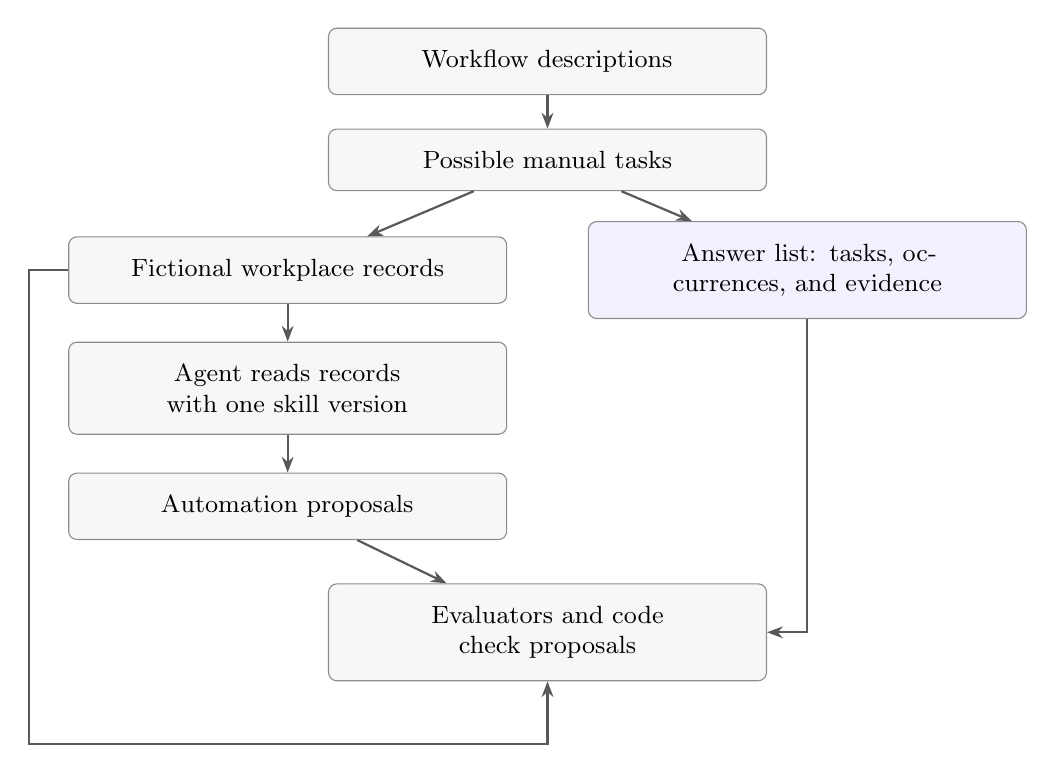
\begin{tikzpicture}[
  box/.style={draw=black!45,rounded corners=3pt,fill=black!3,
    text width=5cm,align=center,inner sep=8pt,font=\small},
  flow/.style={-{Stealth[length=2mm]},thick,draw=black!65}]
\node[box] (source) at (0,0) {Workflow descriptions};
\node[box] (tasks) at (0,-1.25) {Possible manual tasks};
\node[box] (records) at (-3.3,-2.65) {Fictional workplace records};
\node[box,fill=blue!5] (answers) at (3.3,-2.65) {Answer list: tasks, occurrences, and evidence};
\node[box] (reader) at (-3.3,-4.15) {Agent reads records with one skill version};
\node[box] (proposals) at (-3.3,-5.65) {Automation proposals};
\node[box] (checks) at (0,-7.25) {Evaluators and code check proposals};
\draw[flow] (source) -- (tasks);
\draw[flow] (tasks) -- (records);
\draw[flow] (tasks) -- (answers);
\draw[flow] (records) -- (reader);
\draw[flow] (reader) -- (proposals);
\draw[flow] (proposals) -- (checks);
\draw[flow] (answers.south) |- (checks.east);
\draw[flow] (records.west) -- ++(-0.5,0) |- ([yshift=-0.8cm]checks.south) -- (checks.south);
\end{tikzpicture}
\caption{The agent reads workplace records. The answer list is kept for scoring. The checks use the proposals, the records, and the answer list.}
\end{figure}
The plan called for companies with zero, one, three, or five tasks. We could use fewer tasks if the source descriptions did not support enough distinct operations. Companies with zero tasks tested whether the agent would return no proposals when it found no supported manual task, although their activity still included routine discussion and work done by software.

\subsection{Check the generated records before using them}
Code checked the record structure, dates, links, and task annotations, as well as who performed an action and how a field was changed. This distinction mattered: a service changing a Salesforce field is not evidence that a person copied it by hand.

We also checked that records linked to valid sources and did not copy protected source text. A candidate company entered the test only after these checks passed.

For each selected workflow group, we allowed at most four attempts to generate valid activity. When an attempt failed, the model received the previous activity and the validation error so it could repair the problem. A group that still failed was excluded rather than replaced by a different group.

For the first final test, we started with 80 selected groups. Of these, 57 produced valid fictional companies and 23 did not. Creating them required 175 attempts, including 118 rejected attempts. The 57 accepted companies contained 105 known tasks and 4,844 activity records, and eighteen of them had no task on the answer list.

Before running the test, we fixed the list of companies and their contents, which prevented us from adding easier cases, removing difficult cases, or changing their answers after seeing the results.

The failed construction cases still matter, because the reported gains describe the 57 accepted companies and do not establish the same gains across all 80 selected groups. Appendix B shows how the conclusion changes under extreme assumptions about the excluded groups.

\section{Step two: improve the skill's instructions}
\subsection{Use mistakes to identify what the instructions need to explain}
The skill was a text file that told the agent how to read activity, identify tasks, check evidence, and return proposals. We changed that file rather than fine-tuning the language models.

Earlier steps in the study had produced twelve candidate instruction files and 420 assessments across 35 fictional companies. We selected one file as the \textbf{starting skill}. It had the highest report quality among complete candidates that met the required recall and precision thresholds. Those terms are defined in Section 4.

We then ran the starting skill in a development comparison with 59 companies. These were practice cases for improving the instructions, and their records, answer lists, reports, and scores showed where the agent succeeded or failed. We reused these saved materials rather than requesting the same model outputs again.

One recurring error was finding only part of a task. The agent might propose copying a status into a note, while the observed task also required checking the status and opening an issue when it was wrong. That proposal would leave part of the work unexplained.

We divided the 59 companies into two groups: thirty-nine supplied examples for writing revised instructions, and the other twenty were used to choose which revision to test. The companies for the final test were kept outside both groups.

\subsection{Write four candidate instruction files}
We made four requests for revised instructions: two to Claude and two to GPT. Each request included eight practice companies, with two empty answer lists and six nonempty lists, and the model also received the existing instructions, both readers' earlier reports, and feedback on their mistakes.

The requested changes were concrete:

\begin{itemize}
\item Describe the whole observed task, including the result the person produced.
\item Count separate items of work, such as invoices or requests, rather than messages about those items.
\item Cite records that show the person actually doing the work.
\item Explain which part of the work an automation would remove.
\item Allow one supported occurrence to establish a task, while requiring more than one to claim repetition.
\item Return no proposals when the records do not support one.
\end{itemize}

Because the instructions had to apply to other companies, they could not contain company names, record IDs, or answers copied from the practice cases. Otherwise a candidate could memorize the examples instead of learning a useful way to inspect activity.

We also removed a fixed list of permitted task types. The aim was to let evidence determine which tasks qualified, rather than reject a valid task because its category was absent from that list.

\subsection{Choose one revision before the final test}
Both reader models used each valid candidate on the same twenty selection companies, so each candidate had forty scheduled reports.

We selected the candidate with the highest report quality among those that met two minimum conditions. Its recall could be no more than five percentage points below the short comparison prompt. At least 65\% of its returned proposals had to pass the verification checks. Missing judgments contributed zero when candidates were selected.

Three of the four candidates met the thresholds. The selected revision became the \textbf{revised skill} in the first final test, and we fixed its text before that test began. Choosing the winner on practice cases did not count as evidence of improvement on new cases.

Appendix A records the selection scores and the text-length limit that changed during development. The main test compared the complete instruction files rather than isolating the effect of any one sentence or rule.

\section{Step three: test the proposals and explain the scores}
\subsection{Compare three ways to instruct the same readers}
Claude Sonnet 5 and GPT-5.6 Sol each read every test company in three separate runs:

\begin{center}
\small
\setlength{\tabcolsep}{4pt}
\renewcommand{\arraystretch}{1.25}
\begin{tabularx}{\linewidth}{@{}>{\raggedright\arraybackslash}X>{\raggedright\arraybackslash}X@{}}
\toprule
\textbf{Instruction version} & \textbf{What the model received} \\
\midrule
Starting skill & The instruction file used before the first revision. \\
Revised skill & The file selected after learning from the practice cases. \\
Short prompt & A request to find useful automation opportunities, cite evidence, and describe a concrete change. \\
\bottomrule
\end{tabularx}
\end{center}
Every run received the complete activity for the company, the same required report fields, and a limit of five proposals. The same model settings and output limits applied across instruction versions, which made the instructions the main difference within each reader's comparison.

Each company produced six reports: two readers multiplied by three instruction versions. Across 57 companies, this gave 342 reports.

\subsection{Check what each proposal claims}
Every proposal had to describe the work observed, the proposed automation, the trigger, and the item being counted, as well as list separate occurrences with their supporting records. Remaining human work and unknown requirements were reported separately.

We checked two questions separately. First, did the proposal describe one of the tasks on the answer list? Second, did the cited records support its claims about the work, the proposed change, and the count?

Both Claude and GPT acted as evaluators in separate calls. They did not receive the instruction version or the identity of the model that wrote the report, which reduced information that could bias their judgments. Both evaluators had to agree before the relevant claim received a passing score.

Code performed additional checks. Cited records had to exist. The list of work occurrences had to contain distinct items, its citations had to appear in the proposal's evidence, and its length had to match a positive stated count. A verified proposal could not duplicate a known task already matched by another proposal, and the report had to stay within the five-proposal limit.

A proposal was \textbf{verified} only if it passed every evidence and work-removal check. Its count, citations, and list of separate occurrences also had to pass. This was an automated assessment, and it did not mean that a person had approved the proposal or that the automation had been built.

\subsection{Three measures answer different questions}
\textbf{Report quality measures the share of each report that passes verification.} For a nonempty report, we divided the number of verified proposals by the number of returned proposals. Three verified proposals out of four gave that report a quality score of 75\%. We then averaged report scores, and a report with no proposals received zero.

\textbf{Verified task recall measures the share of known tasks found with valid evidence.} If the answer list contained four tasks and verified proposals covered two of them, recall was 50\%. We calculated recall only for companies with at least one task on the answer list, and the measure concerns the tasks we placed in the activity, not every possible automation a real company could have.

\textbf{Pooled precision measures the share of all returned proposals that pass verification.} We added the verified proposals across reports and divided by all proposals returned. For the revised skill in the first test, that was 154 out of 214, or 72.0\%.

Quality and precision use different weights: quality gives each report the same weight, including reports with no proposals, while pooled precision gives each returned proposal the same weight. For example, one perfect one-proposal report and one empty report average 50\% quality, but have 100\% pooled precision.

An empty report can be the right response when there is no supported task, so we recorded that behavior separately. The quality score gave empty reports zero because it measured useful output, not just the avoidance of errors. We also counted \textbf{fully verified reports}: reports with at least one proposal and no proposal that failed verification.

\subsection{Compare results without giving one company extra weight}
We compared instruction versions on the same companies. For each company, we calculated the change for each reader, then averaged those two changes, which prevented a company with more records or proposals from dominating the comparison.

We then used a \textbf{bootstrap} to estimate how much the average change varied across companies. We sampled companies from the test set, with replacement, 10,000 times. For each sample, we recalculated the average paired change, and the middle 95\% of those estimates formed the reported interval.

An interval entirely above zero supports a positive average change under this analysis. An interval that crosses zero does not establish which version is better on that measure. The interval is not a probability that one individual proposal is correct, nor does it measure variation across all possible language models or live companies.

We used a fixed random starting value, called a seed, to make the sampling and job order repeatable, though the seed number itself is not evidence of a better result.

\subsection{Set the pass rule before looking at the test results}
For the revised skill to pass against the starting skill, the lower end of the 95\% interval had to be above zero for \textbf{both quality and recall}. Better recall alone was insufficient: finding more work should not be counted as a joint improvement if report quality did not also improve.

The comparison with the short prompt had a separate rule. Quality had to improve, and the recall interval had to rule out a loss of five percentage points or more. A win against the starting skill did not imply a win against the short prompt.

We also specified how to handle failures. If a reader failed to produce a report after its allowed attempts, the report received zero. If an evaluator failed to return a usable judgment, the judgment stayed missing. We checked whether a conclusion survived treating missing judgments against the revised skill. A timeout or invalid response was not silently treated as a successful proposal.

\section{First test: the revised skill found more known work}
All 342 reports had complete reader and evaluator results, with 114 reports for each instruction version, across 39 companies with known tasks and 18 with none.

\begin{center}
\small
\setlength{\tabcolsep}{4pt}
\renewcommand{\arraystretch}{1.25}
\begin{tabularx}{\linewidth}{@{}>{\raggedright\arraybackslash}X>{\raggedright\arraybackslash}X>{\raggedright\arraybackslash}X>{\raggedright\arraybackslash}X>{\raggedright\arraybackslash}X>{\raggedright\arraybackslash}X@{}}
\toprule
\textbf{Instruction version} & \textbf{Mean report quality} & \textbf{Verified task recall} & \textbf{Pooled precision} & \textbf{Reports with proposals} & \textbf{Fully verified reports} \\
\midrule
Starting skill & 44.7\% & 28.2\% & 74.5\% & 73 of 114 & 43 of 114 \\
Revised skill & 53.0\% & 51.7\% & 72.0\% & 89 of 114 & 50 of 114 \\
Short prompt & 47.1\% & 33.9\% & 55.6\% & 108 of 114 & 28 of 114 \\
\bottomrule
\end{tabularx}
\end{center}
Against the starting skill, the revised skill gained 8.3 percentage points in quality and 23.5 points in recall. Both intervals were above zero, so the revision passed the planned improvement rule.

\begin{center}
\small
\setlength{\tabcolsep}{4pt}
\renewcommand{\arraystretch}{1.25}
\begin{tabularx}{\linewidth}{@{}>{\raggedright\arraybackslash}X>{\raggedright\arraybackslash}X>{\raggedright\arraybackslash}X@{}}
\toprule
\textbf{Comparison} & \textbf{Quality change, 95\% interval} & \textbf{Recall change, 95\% interval} \\
\midrule
Revised skill minus starting skill & +8.3 points [0.3, 16.8] & +23.5 points [13.0, 34.4] \\
Revised skill minus short prompt & +5.8 points [-2.7, 14.8] & +17.8 points [5.6, 30.0] \\
\bottomrule
\end{tabularx}
\end{center}
The revised skill also found more known tasks than the short prompt. However, its quality interval against that prompt crossed zero. We therefore did not establish the planned joint advantage over the short prompt.

The revised skill returned proposals in 77 of the 78 runs on companies with known tasks. It also returned proposals more often on companies with no known task. On those empty-answer companies, the starting skill returned no proposals in all 36 runs. The revised skill did so in 24 runs and the short prompt in six, which shows why output volume alone cannot establish better discovery.

The revised skill's pooled precision was slightly lower than the starting skill's: 72.0\% versus 74.5\%. Its higher mean report quality and recall therefore do not mean that every measure improved.

\subsection{What changed in one successful report}
One test case involved processing website inquiries, where the complete manual task was to review each inquiry and create matching records in Salesforce and Iterable, a marketing platform.

The starting skill proposed Salesforce lead creation and Iterable profile creation separately. Each proposal passed the evidence checks, but neither described the whole known task. The revised skill produced one proposal covering validation, duplicate checks, and creation in both systems. Both evaluators matched it to the complete task.

The records supported three separate inquiries. Ten records helped explain them, but the proposal counted three inquiries, not ten pieces of evidence. It also kept uncertain or duplicate submissions for a person to review.

This example illustrates a difference in the reports, but it does not establish that the task rule alone caused the overall gain, because we tested the revised instruction file as a whole.

\section{Step four: run a second round of instruction improvement}
\subsection{Generate and compare more versions of the skill}
We next tried to improve the revised skill for ten hours, in another round of instruction editing within the study, with the goal of finding a better version of the skill's text.

The 59 earlier development companies and the 57 companies from the first test became 116 practice companies for this round. Reusing the first test as practice did not change its earlier result, although it did mean that those companies could no longer provide an independent test of the new changes. We therefore selected new companies for validation and the second final test.

Each editing round asked a model for two alternative instruction files. We chose two so the process had more than one candidate to compare, though we did not test whether two was the best number.

Both readers tried each valid candidate on 24 practice companies: eight without known tasks and sixteen with known tasks. A promising candidate received another assessment on 24 different practice companies before replacing the current version.

We ranked candidates using the \textbf{harmonic mean} of quality and recall. This is a combined score that falls when either measure is low. For example, 80\% quality with 20\% recall gives a harmonic mean of 32\%, while 50\% on both gives 50\%, which discouraged a candidate from getting a high rank through only one strong measure. We also required minimum precision and limited how much either measure could fall.

The process completed 62 editing rounds and retained two successive instruction changes. The first required a full list of possible tasks before choosing the final proposals, with one consistent item to count for each task. The second allowed a short first-person completion note to support one occurrence. It also required another evidence check before returning an empty report.

These were changes to complete instruction files, and we did not test the individual rules separately. Appendix A gives the candidate counts and the exact selection thresholds.

\subsection{Select a candidate on new companies, then test it once more}
Before the ten-hour editing process, we selected 80 new source groups for validation and 160 for the final test. Each group reserved a place for one fictional company. We excluded previously used groups and matching workflow descriptions.

We generated the validation and test activity only after instruction editing ended, so the model that wrote the instructions did not receive those new records. The same construction checks accepted 60 validation companies and 116 final-test companies, and failed groups were not replaced.

\begin{center}
\small
\setlength{\tabcolsep}{4pt}
\renewcommand{\arraystretch}{1.25}
\begin{tabularx}{\linewidth}{@{}>{\raggedright\arraybackslash}X>{\raggedright\arraybackslash}X>{\raggedright\arraybackslash}X>{\raggedright\arraybackslash}X>{\raggedright\arraybackslash}X@{}}
\toprule
\textbf{Role} & \textbf{Groups selected} & \textbf{Valid fictional companies} & \textbf{Known tasks} & \textbf{Activity records} \\
\midrule
Choose a candidate & 80 & 60 & 109 & 5,045 \\
Test the chosen candidate & 160 & 116 & 208 & 10,088 \\
\bottomrule
\end{tabularx}
\end{center}
We saved the current instruction version every 75 minutes during editing, but the eight saved points contained only two distinct revisions. We compared both revisions with the first-round skill on the 60 validation companies.

\begin{center}
\small
\setlength{\tabcolsep}{4pt}
\renewcommand{\arraystretch}{1.25}
\begin{tabularx}{\linewidth}{@{}>{\raggedright\arraybackslash}X>{\raggedright\arraybackslash}X>{\raggedright\arraybackslash}X>{\raggedright\arraybackslash}X@{}}
\toprule
\textbf{Instruction version} & \textbf{Mean report quality} & \textbf{Verified task recall} & \textbf{Pooled precision} \\
\midrule
First-round skill & 53.1\% & 54.4\% & 72.2\% \\
First candidate from round two & 52.3\% & 51.9\% & 72.7\% \\
Second candidate from round two & 61.8\% & 62.9\% & 77.1\% \\
\bottomrule
\end{tabularx}
\end{center}
The second candidate passed the selection conditions. We fixed its text and compared it with the first-round skill on the 116 final-test companies. Selection results were used to choose the candidate; this last comparison tested whether its gains held on different companies.

\subsection{Second test: recall rose, but the candidate did not pass}
Both readers used both instruction versions on all 116 companies, giving 464 scheduled reports. The new candidate produced 232 complete reports, while the first-round skill produced 230 and had two failures, which received zero. There were no missing evaluator scores.

\begin{center}
\small
\setlength{\tabcolsep}{4pt}
\renewcommand{\arraystretch}{1.25}
\begin{tabularx}{\linewidth}{@{}>{\raggedright\arraybackslash}X>{\raggedright\arraybackslash}X>{\raggedright\arraybackslash}X>{\raggedright\arraybackslash}X>{\raggedright\arraybackslash}X@{}}
\toprule
\textbf{Instruction version} & \textbf{Mean report quality} & \textbf{Verified task recall} & \textbf{Pooled precision} & \textbf{Fully verified reports} \\
\midrule
First-round skill & 59.3\% & 59.2\% & 76.0\% & 117 of 232 \\
Selected round-two candidate & 58.1\% & 65.9\% & 72.4\% & 100 of 232 \\
\bottomrule
\end{tabularx}
\end{center}
The candidate's recall gain was 6.8 percentage points, with a 95\% interval of [0.3, 13.0]. Its quality change was -1.2 points, with an interval of [-6.4, 4.1]. The recall interval was positive, while the quality interval included both a decrease and an increase.

The candidate returned 619 proposals, of which 448 were verified, while the first-round skill returned 441, of which 335 were verified. The candidate therefore found more verified work, but also returned more proposals that failed the checks. Its pooled precision fell, and it produced fewer fully verified reports.

Before the test, we had required positive quality and recall intervals to replace the first-round skill. We had also required no observed decrease in several checks, including pooled precision and fully verified reports, for each reader and overall, and the candidate did not meet those conditions. \textbf{We kept the first-round skill for the distributed package.}

The two final tests used different companies and different comparison versions, so their gains must not be added. Appendix B reports each reader separately and shows the effects of the excluded construction cases.

\section{How we checked the evaluation, and what remains uncertain}
\subsection{Test the evaluators on cases with known expected answers}
Before using the evaluator scores, we tested their behavior on 84 constructed cases with answers specified in the evaluation code, where the test code contained twelve base examples and made seven versions of each. These included a correct proposal, a paraphrase, an unrelated task, a change that did not remove the work, wrong evidence, missing evidence, and a wrong count.

For example, one test stated that a person entered one invoice and later discussed the same invoice. A proposal that counted six invoices should fail the count check. Another test changed a valid automation into an alert telling the person to keep doing the same task by hand. That version should fail the work-removal check.

Across both evaluator models and the relevant decision fields, there were 528 decisions. Of these, 519 matched the specified answers. Three valid task matches and five valid count decisions were missed. One case with invalid evidence received an "unknown" decision. None of the expected negative or unknown cases received a positive decision.

We specified the expected answers in the study's tests rather than collecting ratings from independent users. We reused the control results because the evaluator instructions, models, and scoring rules were unchanged.

\subsection{Check calculations against saved outputs}
We recalculated the reported scores from saved proposals, evidence, and evaluator decisions. We also checked that the test records had not changed. This was a calculation and file-consistency check; it did not establish that every model judgment was correct.

The first comparison's audit reconstructed 342 final-test scores and 240 development scores. The second round's audit reconstructed 360 validation scores and 464 final-test scores, including the two failed reports, and the final numerical analyses matched the stored results.

This paper explains the method and reports aggregate results, but it does not provide the private workflow export or a downloadable copy of the study activity, so readers cannot independently repeat the complete study from this paper alone. We do not treat internal replay checks as a substitute for that access.

\subsection{Limits of the result}
The workplace records were generated. They simulated real work, but they were not observations of people using the skill in live teams, so the test measured whether an agent could recover tasks from those records and support its proposals.

The accepted companies also passed a particular set of construction checks. Rejected cases may differ in ways that matter. The results apply directly to the accepted cases; the sensitivity results in Appendix B show why broader claims would be uncertain.

The readers and evaluators came from the same two model families used during development. Using two evaluators did not make their errors independent. There were no completed human ratings of the final proposals, and the reported intervals did not cover uncertainty from choosing different models.

Because the study changed several instruction rules together, it supports a comparison between complete skill versions but does not establish that the taxonomy alone, or any single new rule, caused the gain. An earlier controlled development comparison did not show a clear advantage for taxonomy feedback over feedback about evidence alone; Appendix A retains that result.

Finally, a supported task is not automatically a task worth automating. The study did not measure user demand, time saved, deployment cost, or reliable operation after deployment. A live workflow still needs the user's decision, access to the relevant systems, field mappings, and appropriate handling of uncertain cases.

\section{Conclusion}
We used existing workflow descriptions to define possible manual tasks, generated activity around those tasks, and used the agent's mistakes to improve its instructions. A separate test showed that the first revised skill produced higher average report quality and found more known tasks than the starting skill.

The second round found a candidate with higher recall, but its report quality did not clearly improve and its precision fell. We kept the first-round skill because the replacement rule required improvement in both quality and recall.

The next question is whether these proposals help people choose useful automations in their own work. That requires evaluation with users and live activity, including the proposals they reject and the work that remains after a workflow is built.

\clearpage
\appendix
\section{How we selected instruction versions}
\subsection{Development before the first final test}
The starting skill was selected from twelve earlier candidates. A candidate needed complete scores, verified recall of at least one third, and pooled precision of at least 70\%. Among candidates that met those conditions, we chose the one with the highest report quality.

The next development step compared the starting skill and the short prompt on 59 companies. The starting skill had 43.2\% quality and 19.6\% recall; the short prompt had 50.2\% quality and 45.2\% recall. This result supplied mistakes to study, but it did not establish that the starting skill was better.

We then used 39 of those companies to write four revisions and twenty to select one. The following table shows the selected revision and its references on those same twenty selection companies. Each row had forty reports, and recall used the fourteen companies with known tasks.

\begin{center}
\small
\setlength{\tabcolsep}{4pt}
\renewcommand{\arraystretch}{1.25}
\begin{tabularx}{\linewidth}{@{}>{\raggedright\arraybackslash}X>{\raggedright\arraybackslash}X>{\raggedright\arraybackslash}X>{\raggedright\arraybackslash}X@{}}
\toprule
\textbf{Version on selection cases} & \textbf{Mean report quality} & \textbf{Verified task recall} & \textbf{Pooled precision} \\
\midrule
Starting skill & 50.4\% & 22.1\% & 76.8\% \\
Selected revision & 58.2\% & 46.0\% & 77.2\% \\
Short prompt & 46.8\% & 49.0\% & 56.1\% \\
\bottomrule
\end{tabularx}
\end{center}
During development, we changed the maximum instruction length from 7,000 to 9,000 characters, which admitted three complete drafts that had already been saved, and we reused their text without another rewrite. The lower limit stayed at 1,200 characters. This was a change to development selection before the final test, not a change made after seeing test results.

The selected instruction body contained 7,684 characters, and the same report-format and occurrence-list instructions were added to all comparison versions. The distributed skill retained the tested text. Package metadata, such as its display name, was separate from those instructions.

\subsection{A check on the role of taxonomy feedback}
An earlier development comparison tested feedback based on workflow tasks against feedback about evidence alone. It used twelve paired development runs. Of 35 accepted test companies, 27 had complete quality comparisons and seventeen had complete recall comparisons on nonempty answer lists.

The quality difference was +0.3 points, with a 95\% interval of [-10.3, 10.1], and the recall difference was -0.9 points, with an interval of [-9.1, 7.0]. It did not pass its improvement rule. We therefore attribute the main result to the complete revised skill, not to a proven effect of taxonomy feedback alone.

\subsection{Candidate selection during the second round}
During the ten-hour editing period, the process created 126 draft plans and obtained 71 valid drafts. Forty-six plans exceeded the allowed input size. Nine others failed the required instruction format after their permitted attempts. The last planned round ended when the time limit was reached.

We reconstructed all 4,121 training scores, including one failed report scored as zero. Previously saved outputs supplied 154 training assessments without new model calls.

To replace the current version during practice, a candidate needed complete scores, at least 65\% pooled precision, and a harmonic-mean gain above 0.005. The last threshold used a 0-to-1 scale, equivalent to more than half a percentage point on a 0-to-100 scale. Quality and recall could each fall by at most three points in the first check and two in the second check.

Two revisions passed this practice rule. Each row below comes from a different second-check group of 24 companies, and the values show the current version followed by its proposed replacement. These are selection results, and the gains cannot be added.

\begin{center}
\small
\setlength{\tabcolsep}{4pt}
\renewcommand{\arraystretch}{1.25}
\begin{tabularx}{\linewidth}{@{}>{\raggedright\arraybackslash}X>{\raggedright\arraybackslash}X>{\raggedright\arraybackslash}X>{\raggedright\arraybackslash}X@{}}
\toprule
\textbf{Retained change} & \textbf{Report quality} & \textbf{Verified task recall} & \textbf{Pooled precision} \\
\midrule
First instruction change & 57.3\% $\rightarrow$ 65.1\% & 52.9\% $\rightarrow$ 71.9\% & 79.8\% $\rightarrow$ 82.7\% \\
Second instruction change & 56.6\% $\rightarrow$ 62.2\% & 53.3\% $\rightarrow$ 61.9\% & 76.3\% $\rightarrow$ 77.4\% \\
\bottomrule
\end{tabularx}
\end{center}
On the 60 new validation companies, a candidate had to match or exceed the first-round skill in quality and recall. It also needed at least 65\% precision, a harmonic-mean gain above 0.005, and complete scores. At most one candidate could be selected. The second candidate passed, and its 7,428-character instruction body was fixed before the last test.

\section{Test composition and uncertainty}
\subsection{Where the fictional records appeared}
\begin{center}
\small
\setlength{\tabcolsep}{4pt}
\renewcommand{\arraystretch}{1.25}
\begin{tabularx}{\linewidth}{@{}>{\raggedright\arraybackslash}X>{\raggedright\arraybackslash}X>{\raggedright\arraybackslash}X>{\raggedright\arraybackslash}X@{}}
\toprule
\textbf{Simulated tool} & \textbf{First final test} & \textbf{Second-round validation} & \textbf{Second final test} \\
\midrule
Slack & 1,625 & 1,864 & 3,626 \\
Notion & 922 & 921 & 1,846 \\
Linear & 1,292 & 1,272 & 2,467 \\
Salesforce & 1,005 & 988 & 2,149 \\
Total records & 4,844 & 5,045 & 10,088 \\
\bottomrule
\end{tabularx}
\end{center}
The first test had 45 English and twelve Spanish companies. Twenty-eight followed conversations and 29 followed daily work. Claude generated 21 companies and GPT generated 36. Thirty-eight companies passed on their first activity-generation attempt.

The answer lists contained zero tasks in eighteen companies, one in fifteen, three in fourteen, four in two, and five in eight. These counts sum to 57 companies and 105 tasks.

The second round's validation set had 41 companies with known tasks and nineteen without them. Its final test had 79 with known tasks and 37 without them. In that final test, the candidate returned proposals in all 158 runs on companies with known tasks, and the first-round skill in 155.

Source selection sought sustained use across several business functions. A selected group needed 10--50 workflows across at least three functions, with at least 70\% having ten successful runs. Additional checks required at least ten qualifying workflows across three functions, a 30-day execution span, and a recent successful run. "Recent" meant within 90 days of 3 September 2026. Accounts marked for solo or non-work use were excluded.

These rules describe the selection method. They do not establish that the selected workflows represent all n8n users or all workplace tasks.

\subsection{Results for each reader}
The main analysis first averaged the two readers' changes within each company. The following tables show the readers separately. Every change is in percentage points, followed by its 95\% interval.

\begin{center}
\small
\setlength{\tabcolsep}{4pt}
\renewcommand{\arraystretch}{1.25}
\begin{tabularx}{\linewidth}{@{}>{\raggedright\arraybackslash}X>{\raggedright\arraybackslash}X>{\raggedright\arraybackslash}X>{\raggedright\arraybackslash}X@{}}
\toprule
\textbf{First test comparison} & \textbf{Reader} & \textbf{Quality change} & \textbf{Recall change} \\
\midrule
Revised minus starting skill & Claude & +6.7 [-4.1, 17.5] & +10.6 [-2.6, 23.8] \\
Revised minus starting skill & GPT & +9.8 [-3.8, 23.9] & +36.3 [22.1, 50.4] \\
Revised minus short prompt & Claude & +7.3 [-4.5, 19.6] & +14.2 [0.5, 28.5] \\
Revised minus short prompt & GPT & +4.4 [-9.3, 17.9] & +21.4 [5.5, 37.4] \\
\bottomrule
\end{tabularx}
\end{center}
\begin{center}
\small
\setlength{\tabcolsep}{4pt}
\renewcommand{\arraystretch}{1.25}
\begin{tabularx}{\linewidth}{@{}>{\raggedright\arraybackslash}X>{\raggedright\arraybackslash}X>{\raggedright\arraybackslash}X@{}}
\toprule
\textbf{Second test: candidate minus first-round skill} & \textbf{Quality change} & \textbf{Recall change} \\
\midrule
Claude & +2.0 [-5.3, 9.2] & +10.9 [2.3, 19.7] \\
GPT & -4.4 [-12.3, 3.5] & +2.7 [-6.2, 11.4] \\
\bottomrule
\end{tabularx}
\end{center}
The improvement was not equally clear for both readers. In the first test, both had positive average changes against the starting skill, but several reader-specific intervals crossed zero. In the second test, GPT's average quality change was negative.

\subsection{What if the excluded construction cases had been usable?}
The first test excluded 23 of 80 selected source groups, and the second final test 44 of 160. We could not measure discovery performance on those failed constructions.

To show how much this exclusion could matter, we calculated two extremes. In the adverse case, every missing revised-skill score was zero and every missing reference score was one. In the favorable case, we reversed those values. The requested number of tasks determined whether an excluded case entered the recall calculation.

These are deliberately extreme assumptions. They do not predict the missing results. They show that the positive finding on accepted companies does not establish a positive finding across every selected group.

\begin{center}
\small
\setlength{\tabcolsep}{4pt}
\renewcommand{\arraystretch}{1.25}
\begin{tabularx}{\linewidth}{@{}>{\raggedright\arraybackslash}X>{\raggedright\arraybackslash}X>{\raggedright\arraybackslash}X>{\raggedright\arraybackslash}X@{}}
\toprule
\textbf{First test, including all 80 selected groups} & \textbf{Assumption} & \textbf{Quality change} & \textbf{Recall change} \\
\midrule
Revised minus starting skill & Adverse & -22.9 [-35.4, -10.6] & -19.7 [-35.8, -3.1] \\
Revised minus starting skill & Favorable & +34.6 [23.9, 45.6] & +50.3 [38.6, 61.6] \\
Revised minus short prompt & Adverse & -24.6 [-36.8, -12.6] & -23.4 [-39.4, -7.0] \\
Revised minus short prompt & Favorable & +32.9 [21.6, 44.2] & +46.6 [33.8, 58.9] \\
\bottomrule
\end{tabularx}
\end{center}
\begin{center}
\small
\setlength{\tabcolsep}{4pt}
\renewcommand{\arraystretch}{1.25}
\begin{tabularx}{\linewidth}{@{}>{\raggedright\arraybackslash}X>{\raggedright\arraybackslash}X>{\raggedright\arraybackslash}X@{}}
\toprule
\textbf{Second test, including all 160 selected groups} & \textbf{Quality change} & \textbf{Recall change} \\
\midrule
Adverse assumption & -28.4 [-36.3, -20.5] & -29.7 [-39.8, -19.6] \\
Favorable assumption & +26.6 [18.7, 34.8] & +38.6 [29.6, 47.5] \\
\bottomrule
\end{tabularx}
\end{center}
\subsection{Checks used to decide whether to replace the skill}
The second-round candidate also had to avoid observed decreases on the measures below, both overall and for each reader. The table shows candidate minus first-round skill, in percentage points. These are observed differences, not confidence intervals.

\begin{center}
\small
\setlength{\tabcolsep}{4pt}
\renewcommand{\arraystretch}{1.25}
\begin{tabularx}{\linewidth}{@{}>{\raggedright\arraybackslash}X>{\raggedright\arraybackslash}X>{\raggedright\arraybackslash}X>{\raggedright\arraybackslash}X@{}}
\toprule
\textbf{Measure} & \textbf{Both readers} & \textbf{Claude} & \textbf{GPT} \\
\midrule
Mean report quality & -1.2 & +2.0 & -4.4 \\
Verified task recall & +6.8 & +10.9 & +2.7 \\
Pooled precision & -3.6 & -5.6 & -2.6 \\
Fully verified report rate & -7.3 & -3.4 & -11.2 \\
Reports with proposals on companies with known tasks & +1.9 & +3.8 & +0.0 \\
\bottomrule
\end{tabularx}
\end{center}
Several checks failed. We did not treat the increase in the number of proposals as sufficient reason to replace the skill.

\section{Model settings and calculation details}
The same settings applied to the compared instruction versions. Limits are shown here so readers can distinguish changes to the instructions from changes to the model setup.

\begin{center}
\small
\setlength{\tabcolsep}{4pt}
\renewcommand{\arraystretch}{1.25}
\begin{tabularx}{\linewidth}{@{}>{\raggedright\arraybackslash}X>{\raggedright\arraybackslash}X@{}}
\toprule
\textbf{Setting} & \textbf{Value used} \\
\midrule
Readers and evaluators & Claude Sonnet 5 and GPT-5.6 Sol \\
Claude thinking & Disabled \\
GPT reasoning effort & Low \\
Temperature & No override \\
Maximum proposals in a report & Five \\
Report output limit & 16,000 tokens \\
Evaluator output limit & 8,000 tokens \\
Activity-generation output limit & 32,000 tokens \\
Attempts per reader or evaluator call & At most two \\
Concurrent final-test calls & At most six per provider \\
\bottomrule
\end{tabularx}
\end{center}
A token is a unit of text processed by the model. The output limits capped how much text a call could return, and were not counts of tasks or activity records.

The improvement rules and failure treatment were fixed before test outputs were available. We inspected test performance after every scheduled report had either completed or failed, which prevented us from stopping after a favorable partial result.

There were two planned joint claims in the first test: improvement over the starting skill and superiority to the short prompt. Each required two conditions to pass, and the lower ends of two-sided 95\% intervals corresponded to nominal one-sided error of 2.5\% per joint claim. Across the two claims, the nominal error bound was 5\%. Bootstrap coverage is approximate, so this is a design-level error bound rather than a guarantee.

For missing evaluator scores, the adverse analysis assigned zero to the revised skill and one to its reference, while the favorable analysis did the reverse. Neither final test had missing evaluator scores, so these analyses gave the same estimates as the complete-score analysis. Failed reader reports remained zero as specified.

All displayed percentages and differences are rounded separately from the underlying calculations. Subtracting two displayed percentages can therefore differ by 0.1 points from the displayed paired change. For example, the second test's reported recall gain was 6.8 points even though its rounded means were 65.9\% and 59.2\%.

The first round's new model calls had an estimated cost of US\$105.52, including failed attempts. The second round recorded 20,816 calls, with an estimated cost of US\$821.36 and a further unresolved upper bound of US\$2.02 for eight interrupted calls. These figures exclude previously saved outputs reused in the study, and describe study execution costs, not the cost of running the skill for a user.

\section*{Related work and references}
WorkArena evaluates agents on tasks assigned to them [1]. This study instead asked an agent to identify possible tasks from mixed activity. Process mining and robotic process mining also study how work can be recovered from event or interaction records [2, 3].

Work on instruction optimization provides methods for improving a text prompt from task feedback [4--6]. We applied this idea to a skill that proposes automations. Research on citation support and model-based evaluation also motivates checking what a proposal means separately from whether its evidence supports it [7, 8].

\begin{enumerate}
\item Drouin, Alexandre, Maxime Gasse, Massimo Caccia, et al. 2024. \href{https://proceedings.mlr.press/v235/drouin24a.html}{WorkArena: How Capable Are Web Agents at Solving Common Knowledge Work Tasks?} Proceedings of the 41st International Conference on Machine Learning, 235: 11642--11662.
\item van der Aalst, Wil M. P. 2016. \href{https://doi.org/10.1007/978-3-662-49851-4}{Process Mining: Data Science in Action}. Second edition. Springer.
\item Leno, Volodymyr, Artem Polyvyanyy, Marlon Dumas, Marcello La Rosa, and Fabrizio Maria Maggi. 2021. \href{https://doi.org/10.1007/s12599-020-00641-4}{Robotic Process Mining: Vision and Challenges}. Business \& Information Systems Engineering 63: 301--314.
\item Zhou, Yongchao, Andrei Ioan Muresanu, Ziwen Han, et al. 2023. \href{https://arxiv.org/abs/2211.01910}{Large Language Models Are Human-Level Prompt Engineers}. International Conference on Learning Representations.
\item Khattab, Omar, Arnav Singhvi, Paridhi Maheshwari, et al. 2024. \href{https://proceedings.iclr.cc/paper_files/paper/2024/hash/f1cf02ce09757f57c3b93c0db83181e0-Abstract-Conference.html}{DSPy: Compiling Declarative Language Model Calls into State-of-the-Art Pipelines}. International Conference on Learning Representations.
\item Pryzant, Reid, Dan Iter, Jerry Li, Yin Lee, Chenguang Zhu, and Michael Zeng. 2023. \href{https://doi.org/10.18653/v1/2023.emnlp-main.494}{Automatic Prompt Optimization with "Gradient Descent" and Beam Search}. Proceedings of EMNLP, 7957--7968.
\item Gao, Tianyu, Howard Yen, Jiatong Yu, and Danqi Chen. 2023. \href{https://doi.org/10.18653/v1/2023.emnlp-main.398}{Enabling Large Language Models to Generate Text with Citations}. Proceedings of EMNLP, 6465--6488.
\item Zheng, Lianmin, Wei-Lin Chiang, Ying Sheng, et al. 2023. \href{https://arxiv.org/abs/2306.05685}{Judging LLM-as-a-Judge with MT-Bench and Chatbot Arena}. Advances in Neural Information Processing Systems, Datasets and Benchmarks Track.
\end{enumerate}
\end{document}
